\documentclass[12pt]{article}
\usepackage{ivanp}
\usepackage{subcaption}
\usepackage{minted}

\title{Higgs + jet angular distributions}
\author{Ivan Pogrebnyak}
\date{\today}

\begin{document}
\maketitle

%%%%%%%%%%%%%%%%%%%%%%%%%%%%%%%%%%%%%%%%%%%%%%%%%%%%%%%%%%%%%%%%%%%%%

\section{Definitions}
The variable of interest is $\cos\theta$ in bins of Hj mass, $M$, where
$\theta$ is the angle between the Higgs momentum and the beam axis (polar angle).

\begin{equation}
  \cos\theta = \frac{p_{z,H}}{ \sqrt{p_{x,H}^2+p_{y,H}^2+p_{z,H}^2} }
\end{equation}
\begin{equation}
  M = \sqrt{(p_H + p_j)^2}
  = \sqrt{(E_H+E_j)^2-(p_{x,H}+p_{x,j})^2-(p_{y,H}+p_{y,j})^2-(p_{z,H}+p_{z,j})^2}
\end{equation}

The idea is to fit, to the $\cos\theta$ distributions, a function of the form
\begin{equation}
  g(\cos\theta) = \normsq{c_0 + \sum_{k=1}^{n}c_{2k}e^{i\phi_{2k}}P_{2k}(\cos\theta)},
\end{equation}
where $P_k$ are Legendre polynomials;
and then perform a statystical test for a hypothesis that $\phi_{2k}\neq0$.

For an initial attempt, consider the case $n=3$, and $\phi_{2k}=0$ for $k>1$.

Absolute value of $\cos\theta$ can be used, as the functions are even.
Even Legendre polynomials are orthogonal on $[0,1]$, since all Legendre
polynomials are orthogonal on $[-1,1]$.

$c_0$ does not represent an independent degree of freedom, and can be
eliminated by normalizing $g$,
\begin{equation}
  1 = \int_0^1 g(x) dx = c_0^2 + \tfrac{1}{5}c_2^2 + \tfrac{1}{9}c_4^2 + \tfrac{1}{13}c_6^2.
\end{equation}

\subsection{\texorpdfstring{\texttt{C++}}{C++} code}
\begin{minted}{cpp}
  double fitf(double* x, double* c) { // c is { c2, c4, c6, phi2 }
    // powers of x
    const double x2 = sq(*x), x4 = x2*x2, x6 = x4*x2;

    // Legendre polynomials
    const double p2 = 1.5*x2 - 0.5;
    const double p4 = 4.375*x4 - 3.75*x2 + 0.375;
    const double p6 = 14.4375*x6 - 19.6875*x4 + 6.5625*x2 - 0.3125;

    const double c0 = std::sqrt(
      1. - (0.2*sq(c[0]) + (1./9.)*sq(c[1]) + (1./13.)*sq(c[2])) );

    const auto phase = exp(std::polar<double>(1.,c[3]));

    // norm squared
    return norm( c0 + c[0]*phase*p2 + c[1]*p4 + c[2]*p6 );
  }
\end{minted}

\section{\texorpdfstring{$\cos\theta$}{cos theta} distributions}
Using the unweighted events I sent to John Ralston
(no photon cuts, 25 GeV pT and 4.5 eta jet cuts).
\begin{figure}[H]
  \centering
  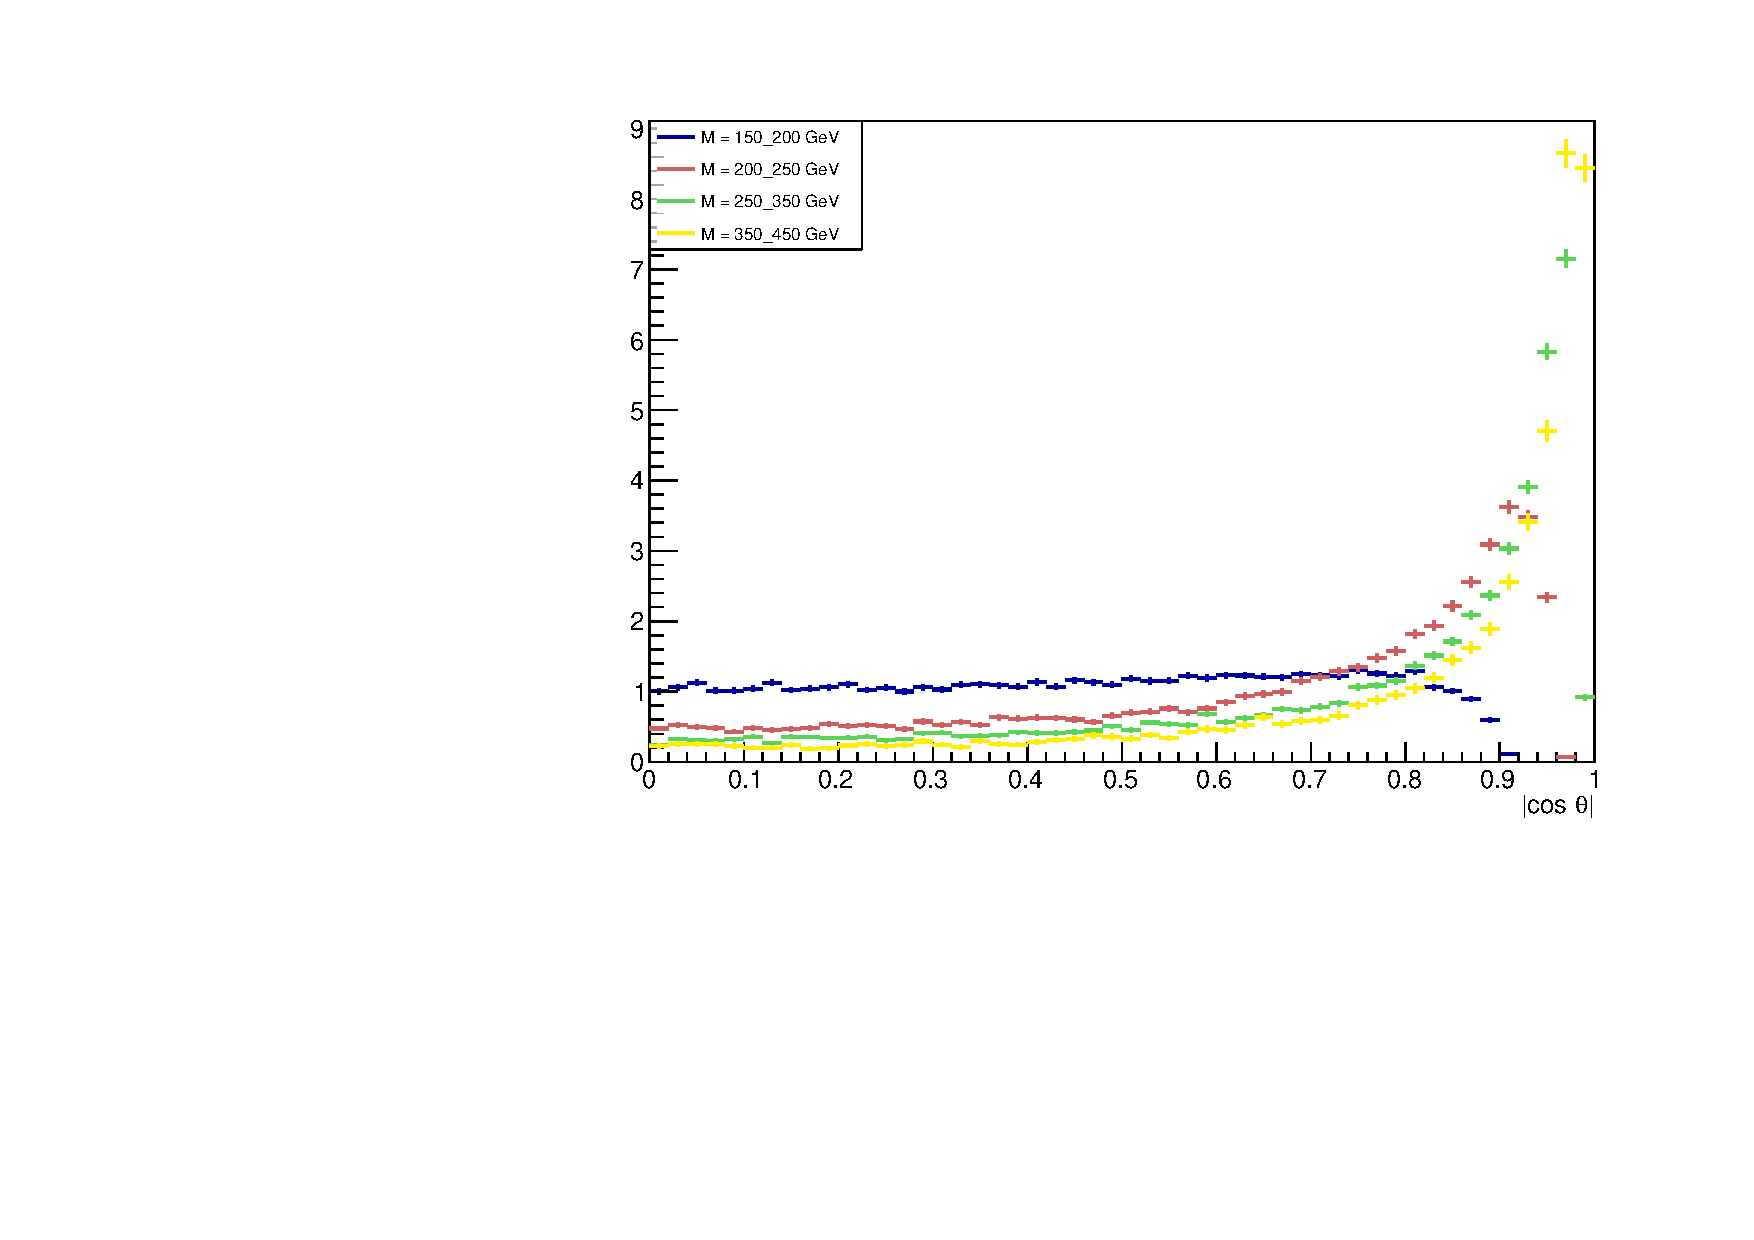
\includegraphics[width=0.75\linewidth]{../1/abs_cos_theta.pdf}
  \caption{Higgs $|\!\cos\theta|$ distribution as a function of mass of the Higgs+jet system}
\end{figure}

\pagebreak

\section{Fits}
Using the events I sent to John Ralston and with fixed $\phi_2 = 0$.

\begin{figure}[H]
  \centering
  \begin{subfigure}[b]{0.49\textwidth}
    \centering
    \caption{$150\leq M_{Hj}<200$}
    \includegraphics[width=\textwidth,trim={10mm 0 10mm 13mm},clip]{../1/150_200_fit.pdf}
  \end{subfigure}
  \begin{subfigure}[b]{0.49\textwidth}
    \centering
    \caption{$200\leq M_{Hj}<250$}
    \includegraphics[width=\textwidth,trim={10mm 0 10mm 13mm},clip]{../1/200_250_fit.pdf}
  \end{subfigure}
  \begin{subfigure}[b]{0.49\textwidth}
    \centering
    \caption{$250\leq M_{Hj}<350$}
    \includegraphics[width=\textwidth,trim={10mm 0 10mm 13mm},clip]{../1/250_350_fit.pdf}
  \end{subfigure}
  \begin{subfigure}[b]{0.49\textwidth}
    \centering
    \caption{$350\leq M_{Hj}<450$}
    \includegraphics[width=\textwidth,trim={10mm 0 10mm 13mm},clip]{../1/350_450_fit.pdf}
  \end{subfigure}
\end{figure}

\pagebreak

\section{GoSam distributions}
With ATLAS jet and photon cuts.

\begin{figure}[H]
  \centering
  \begin{subfigure}[b]{0.8\textwidth}
    \centering
    \caption{Total weight}
    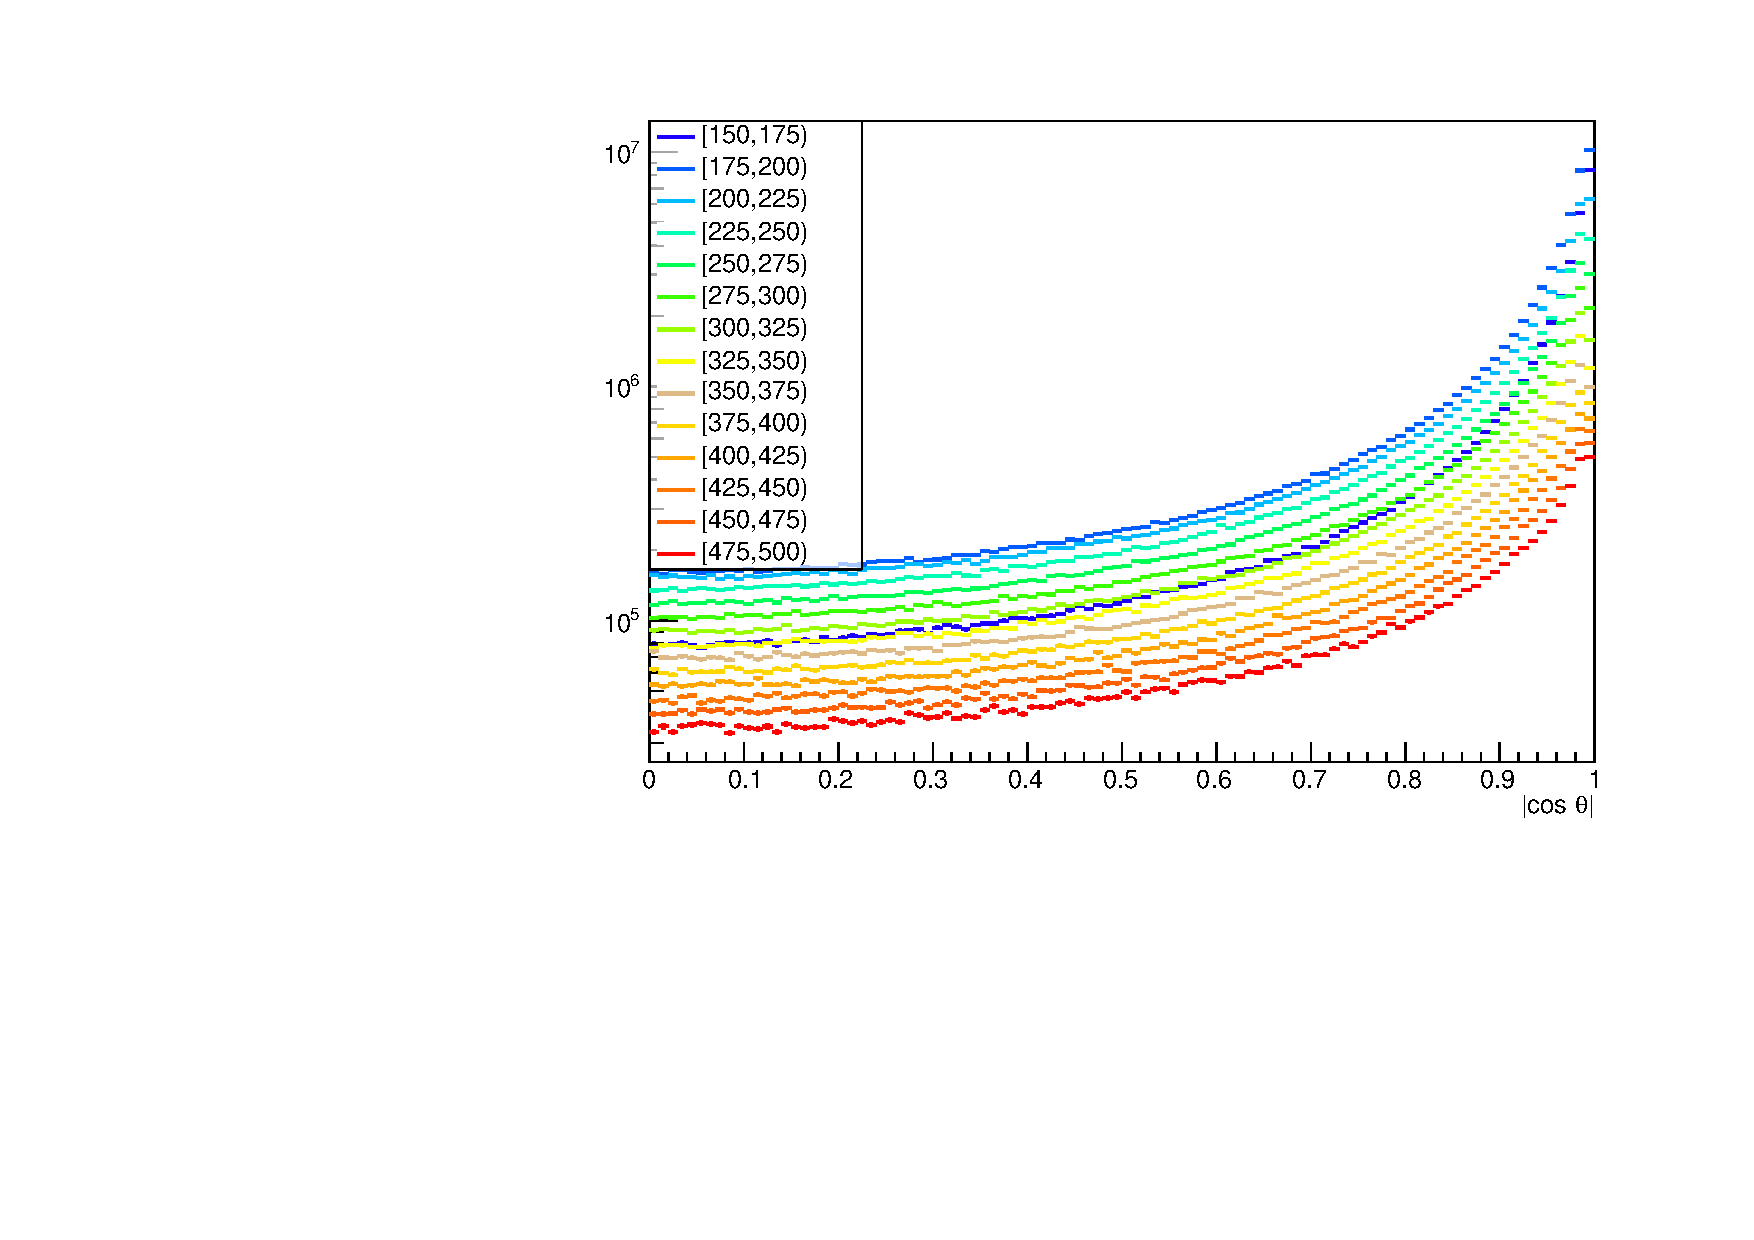
\includegraphics[width=\textwidth,trim={10mm 0 10mm 13mm},clip]{plots/gosam.pdf}
  \end{subfigure}
  \begin{subfigure}[b]{0.8\textwidth}
    \centering
    \caption{Normalized}
    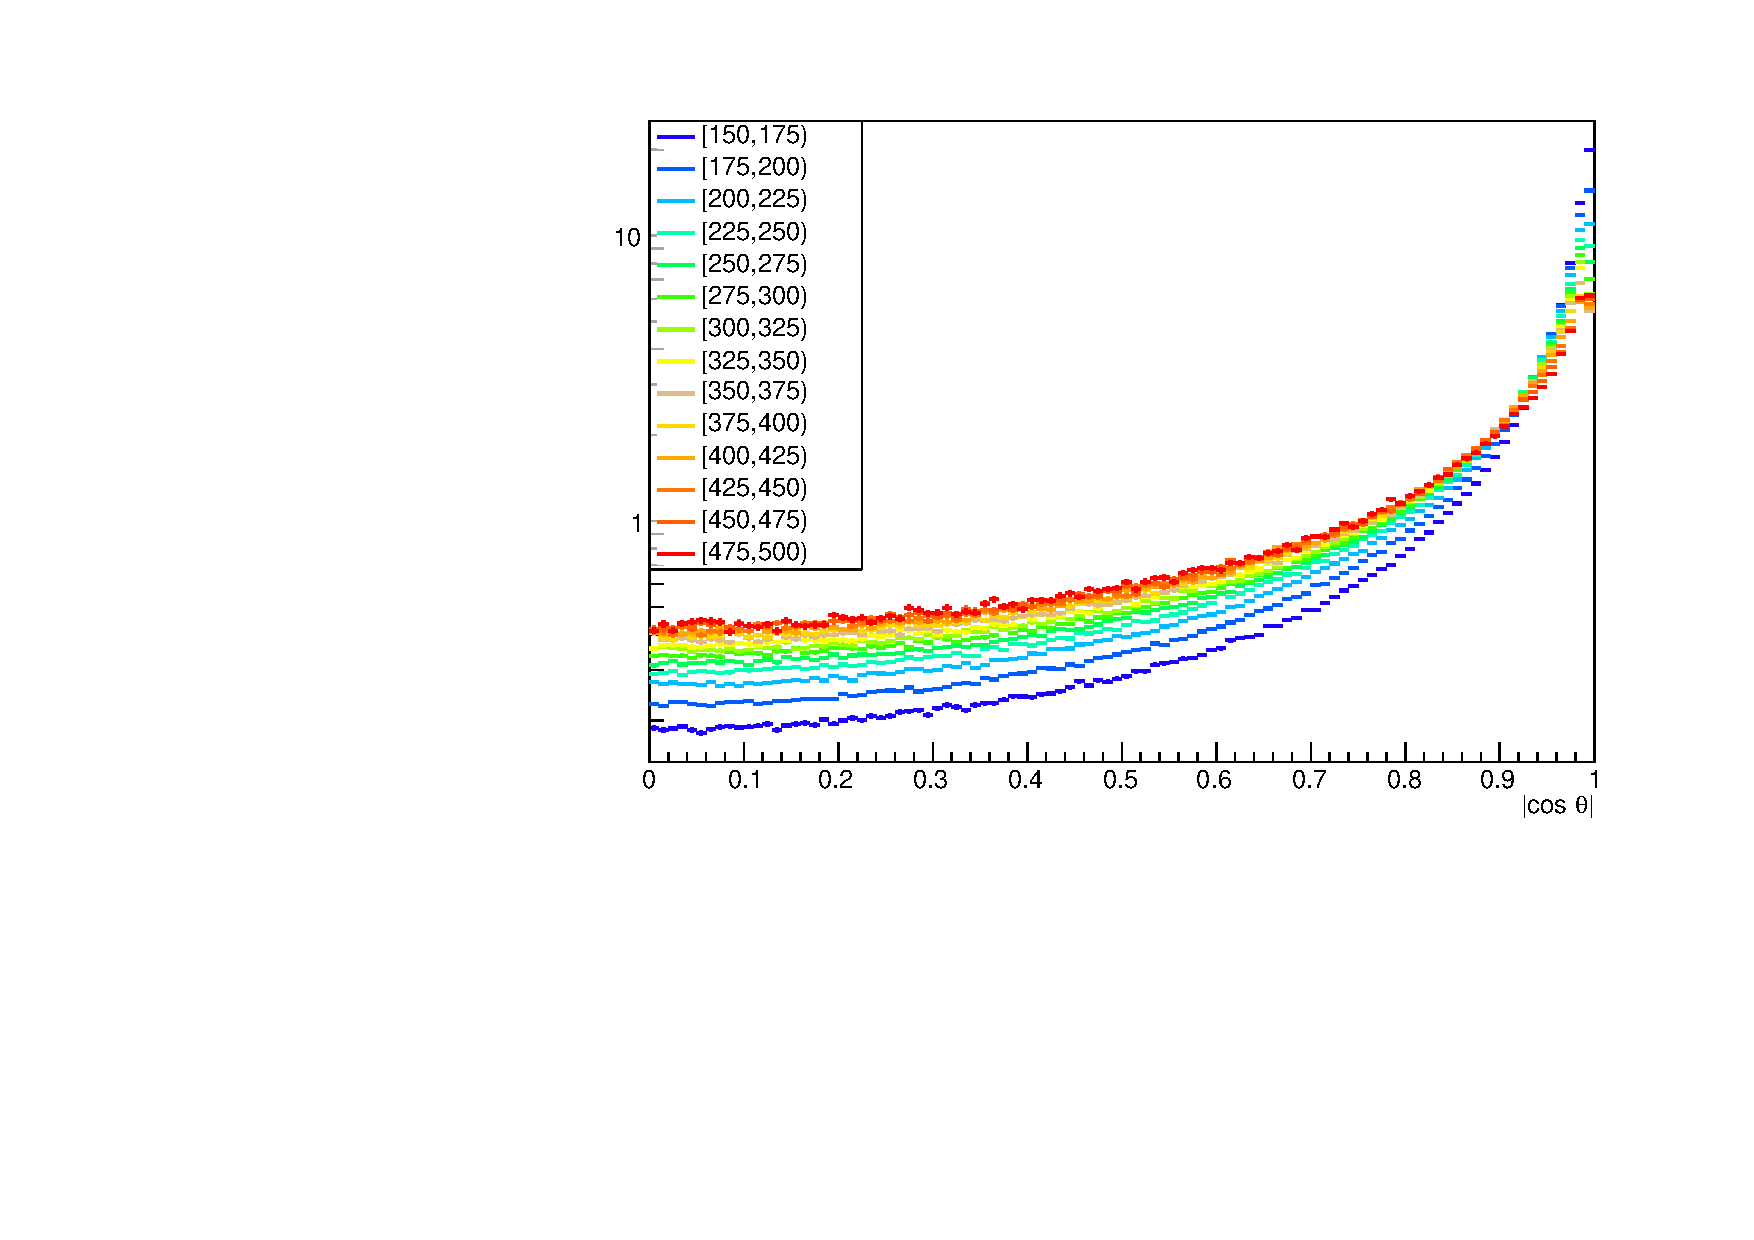
\includegraphics[width=\textwidth,trim={10mm 0 10mm 13mm},clip]{plots/gosam_norm.pdf}
  \end{subfigure}
\end{figure}

\end{document}

